%chap2
\chapter{Analyse et conception}


\thispagestyle{empty}

\newpage

%================header and footer============


\sethead{}{}{Analyse des besoins}\headrule



%==============Début

 \section{Analyse}
 
\subsection{Modèle du cycle de vie}

\subsection{Raffinement des cas d'utilisations}
   
   \subsubsection{Diagramme détaillé de cas d'utilisation <<s'authentifier>>}
   
   \subsubsection{Diagramme détaillé de cas d'utilisation <<demande d'ouverture d'un dossier AVA>>}
  
  \subsubsection{Diagramme détaillé de cas d'utilisation <<Consulter l'avancement des dossiers AVA>>}
   
    \subsubsection{Diagramme détaillé de cas d'utilisation <<Annulation de voyage>>}
    
     \subsubsection{Diagramme détaillé de cas d'utilisation <<Rétrocession>>}
     
     \subsubsection{Diagramme détaillé de cas d'utilisation <<Ajouter un Bénéficiaire>>}
     
      \subsubsection{Diagramme détaillé de cas d'utilisation <<Désactiver un Bénéficiaire>>}
     
 
 \section{Conception}
 
 \subsection{Diagrammes d'activités}
 
 \subsubsection{Diagrammes d'activité << Demande d'exécution d'opérations>>}
 
  \subsubsection{Diagrammes d'activité <<Rétrocession>>}
  
  \subsection{Diagrammes de séquences}
  
  \subsubsection{Diagramme de séquence << s'authentifier>>}
  
  \subsubsection{Diagramme de séquence << Ajouter bénéficiaire>>}
  
  \subsection{Diagramme des classes global}
  
  %inclusion d'une mage dans le document
\begin{figure}[!h]


%remplacer "width" par "height" pour régler la hauteur

\begin{center}
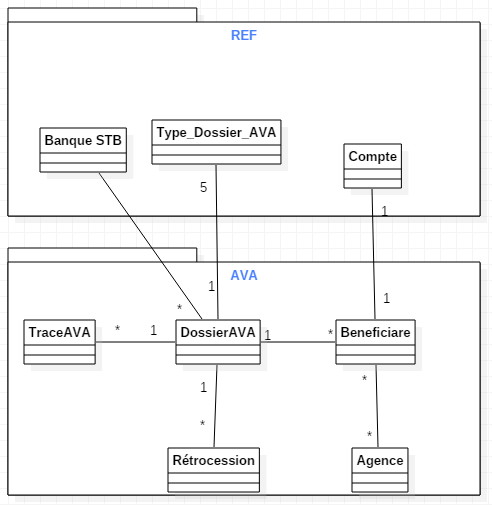
\includegraphics{./conception/diagramme_classes}

%légende de l'image
\caption{Diagramme des classes global}
\end{center}
\end{figure}
  
  
  
  
 

 
 
 

 